%introduction不可直接编译
\section{Introduction}
\subsection{Restatement of the Problem}
Energy is an important support of modern economy. It turns to be the material basis for the survival of human society, and it plays an indispensable role in promoting the economic and social development.\cite{energy} 
With the economic development and fast population growth,the demand for energy grows larger and larger,energy consumption increases substantially,and the traditional energy resources decline day by day,which can not meet the needs of economic development. So the United States in need of new energy to satisfy the increasingly growing demands for energy consumption,in addition,it can construct environmentally friendly country. \\
There are four states – California (CA), Arizona(AZ), New Mexico (NM), and Texas (TX) – that wish to form a realistic new energy compact focused on increased usage of cleaner, renewable energy sources. \\
We need to provide an energy profile for each of the four states using the data given and develop a model to describe how the energy profile. Then we are required to address the results of our model to provide a concise description for the similarities and differences between the four states.We also should select the credible criteria to determine the 'best' profile for usage of cleaner, renewable energy in 2009 and predict the energy profile of each state for 2025 and 2050 in the absence of policy based on the historical development and our understanding of the profile.\\
Then we are supposed to determine renewable energy usage for 2025 and 2050 and necessary actions to meet the goals for new renewable energy compact. Finally, we should prepare a memo to the group of Governors summarizing the state profiles.
\subsection{Overview of Our Work}
The flow chart of the whole model is presented below in \autoref{fig:float}:
\begin{figure}
	\centering
	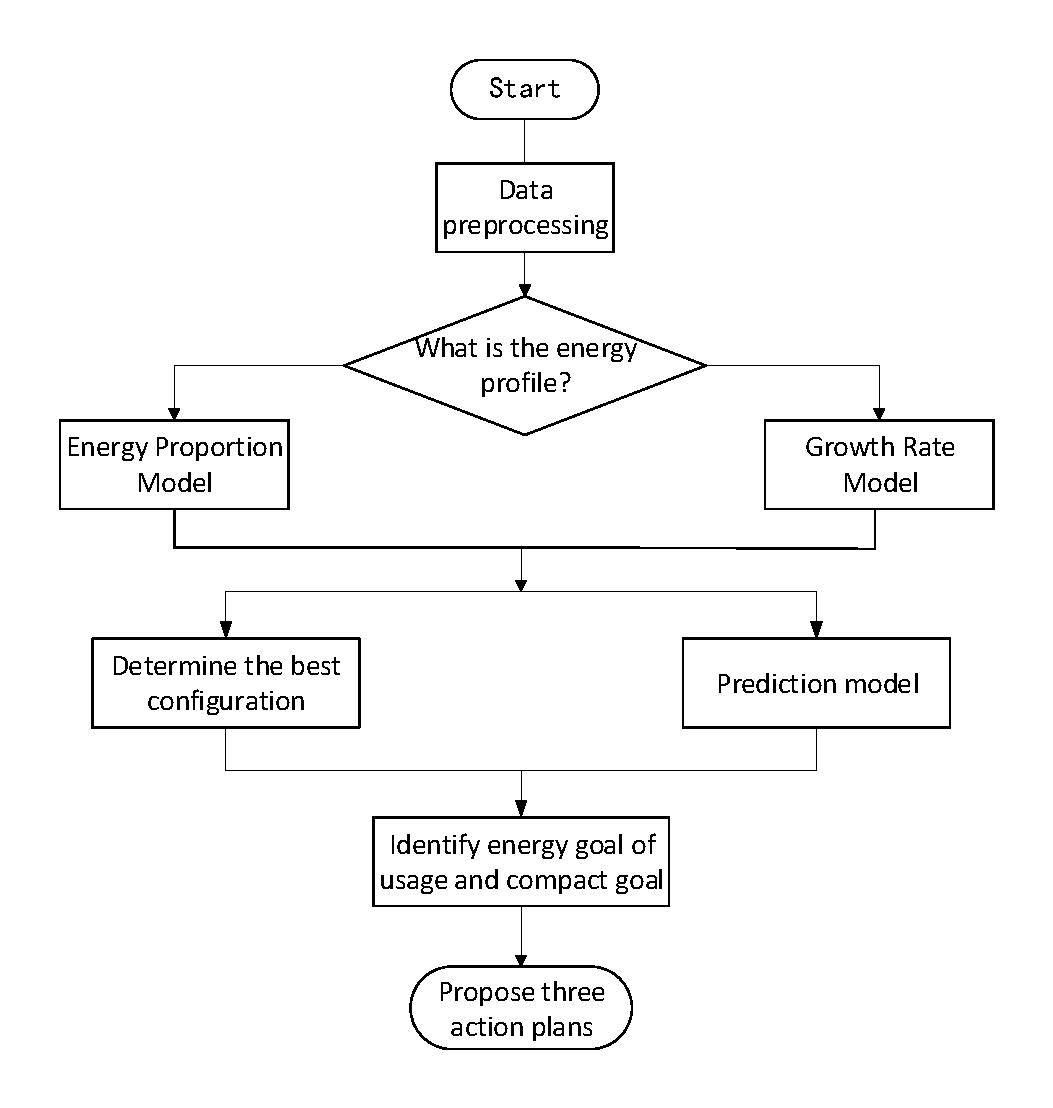
\includegraphics[width=10cm]{figure/float}
	\caption{Flow Chart Demonstration of the Model}
	\label{fig:float}
\end{figure}
